% Generated from export-roundtrip.typ. Typst is authoritative; regeneration overwrites this file.
\documentclass{qlnotes-export}

\title{Probability export round-trip / 概率论导出试验}
\subtitle{One Typst source, editable LaTeX and Markdown}
\author{Qiulin Fan}
\date{2026}

\begin{document}
\frontmatter
\maketitle
\tableofcontents

\mainmatter
\chapter{Joint distributions / 联合分布}

% qlnotes: kind=definition; id=def-joint-support; concepts=joint-distribution, support; depends=random-variable, density; aliases=联合分布支撑集
\begin{definition}{Support / 支撑集}\label{def-joint-support}

The support of a joint density \(f_{X,Y}\) is the set on which \(f_{X,Y}\left( {x,y} \right) > 0\). In the region below, \(\mathbb{P}\left( {\left( {X,Y} \right) \in A} \right)\) is obtained by integrating over \(A\).

\end{definition}

% qlnotes: kind=lemma; id=lem-probability-nonnegative; concepts=probability-measure; depends=measure
\begin{lemma}{Non-negativity}\label{lem-probability-nonnegative}

For every measurable event \(A\), \(\mathbb{P}(A) \geq 0\).

\end{lemma}

\begin{proof}

This follows directly from the codomain of a probability measure.

\end{proof}

% qlnotes: kind=corollary; id=cor-probability-bound; concepts=probability-bound; depends=probability-measure
\begin{corollary}\label{cor-probability-bound}

Every event satisfies \(0 \leq \mathbb{P}(A) \leq 1\).

\end{corollary}

\begin{qlremark}{Remark}

The semantic IDs above are preserved in both exported formats.

\end{qlremark}

\begin{example}[A direct calculation]

If \(\mathbb{P}(A) = \frac{1}{2}\), compute \(\mathbb{P}\left( A^{c} \right)\).

\begin{qlsolution}{Solution}

Since \(A\) and \(A^{c}\) partition the sample space, \(\mathbb{P}\left( A^{c} \right) = 1 - \mathbb{P}(A) = \frac{1}{2}\).

\end{qlsolution}

\end{example}

\begin{center}

\pandocbounded{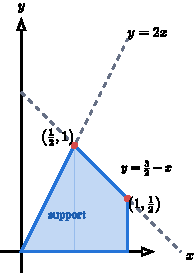
\includegraphics[keepaspectratio,alt={The support region bounded by y equals 2x, y equals three halves minus x, and the x-axis.}]{assets/fig-joint-support.pdf}}

\end{center}

The geometric interpretation is consistent with the standard measure-theoretic development in \autocite{folland1999}.

\printbibliography
\end{document}
